\subsection{PD Regler}
\label{subsec:02PDregler}

Ein einfacher Ansatz f\"ur den Rundkurs ohne Hindernisse ist die Abstandregelung mit Hilfe der Ultraschallsensoren und einem PID Regler. Die zu regelnde Gr\"o\ss{}e ist der Abstand zur Wand, als Stellgr\"o\ss{}e dient der Lenkwinkel. Dazu kann entweder die Stellgr\"o\ss{}e f\"ur den Lenkwinkel geregelt werden oder der Lenkwinkel selbst, welcher dann auf die Stellgr\"o\ss{}e aus dem Lenkwinkelmodell umgerechnet wird. Die Reglerauslegung ist sowohl per Simulation in Simulink als auch experimentell durchgef\"uhrt worden. \\
Die Simulation beruht auf dem Ackermann-Modell, einem Einspurmodell f\"ur Fahrzeuge. Es lautet

\begin{align*} 
	\dot{\varphi}_\text{K} &= \frac{v}{l}\cdot\tan\varphi_\text{L}\\
	\dot{y} &= v \cdot \sin \varphi_\text{K}+v\cdot\frac{l_\text{H}}{l}\cdot\cos\varphi_\text{K}\cdot\tan\varphi_\text{L}.
	\intertext{Durch Linearisierung erh\"alt man}
	\dot{\varphi}_\text{K} &= \frac{v}{l}\cdot\varphi_\text{L}\\
	\dot{y} &= v\cdot\varphi_\text{K}+v\cdot\frac{l_\text{H}}{l}\cdot\varphi_\text{L}.
\end{align*}
Dabei ist $\varphi_\text{K}$ der Kurswinkel, $\varphi_\text{L}$ der Lenkwinkel, $v$ die Geschwindigkeit des Fahrzeugs, $l$ der Achsabstand, $l_\text{H}$ der Abstand von der Hinterachse zu einem Referenzpunkt und $y$ der Abstand zur Wand. Mit beiden Systemen wurde in Simulink eine PD-Reglerauslegung durchgef\"uhrt. Es wurden diskrete Systeme betrachtet (vergleiche Abbildung \ref{fig:regelkreis}), die Geschwindigkeit war $\SI[per-mode=fraction]{0.5}{\meter\per\second}$. Der simulierte Verlauf der Sprungantwort ist in Abbildung \ref{fig:SprungantwortSimulink} dargestellt, der Stellgr\"o\ss{}enverlauf in Abbildung \ref{fig:StellgroesseSimulink}.

\begin{figure}[h]
	\centering
	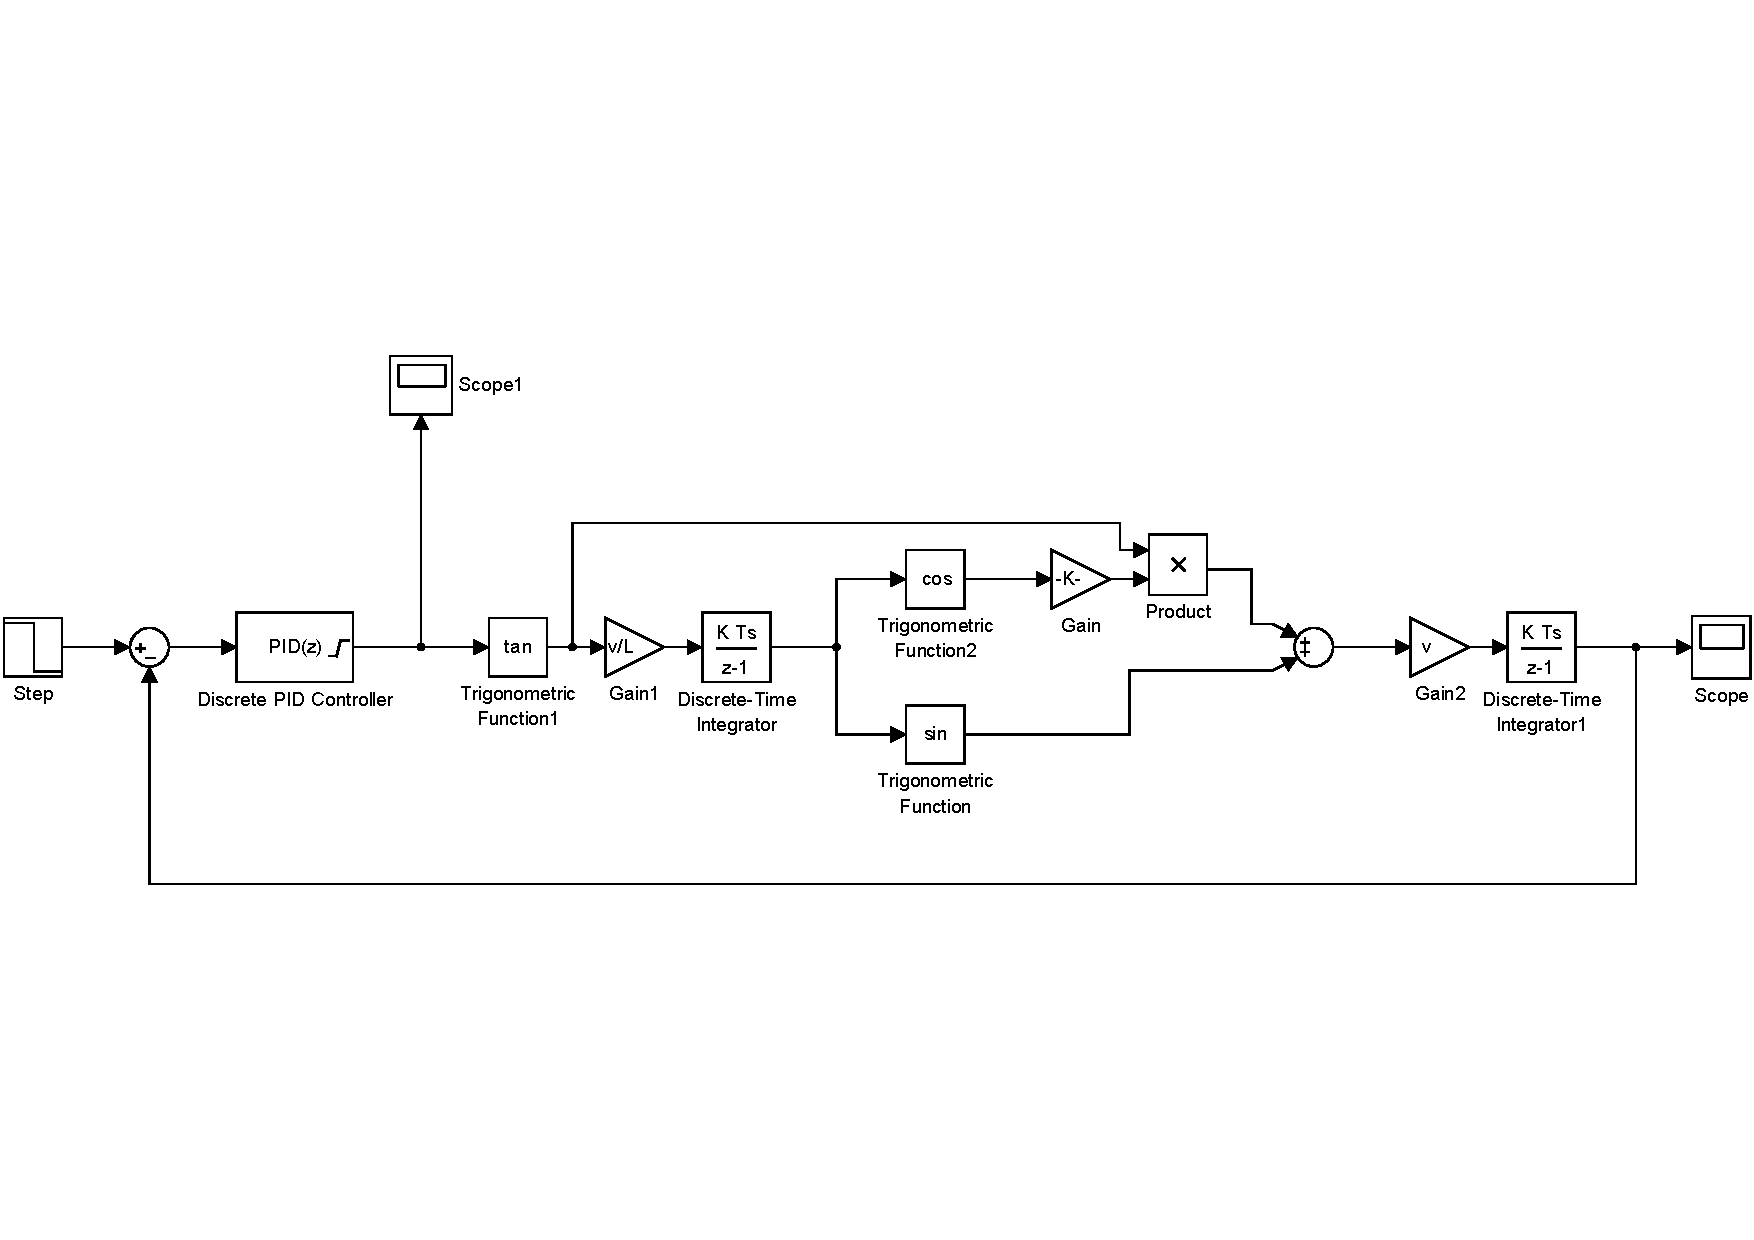
\includegraphics[width=0.9\linewidth,trim=0cm 6cm 0cm 6cm, clip]{pics/system.pdf}
	\caption{Diskreter Regelkreis mit nicht linearisieren Ackermann-Modell.}
	\label{fig:regelkreis}
\end{figure}
\begin{figure}
	\centering
	\subfigure[Sprungantwort]{
			\begin{tikzpicture}
			\begin{axis}[xlabel = Zeit in \si{\second},ylabel=Regelgr\"o\ss{}e in \si{\meter},xmin=0,xmax=9,ymin=0.2, ymax=0.9, axis x line=bottom, axis y line=left,grid,width=7cm,height=5cm]
			\addplot[mark=none,very thick] table [col sep=semicolon] {pics/sprungantwortSimulink.csv};
			\end{axis}
			\label{fig:SprungantwortSimulink}
			\end{tikzpicture}}
	\subfigure[Stellgr\"o\ss{}e]{
			\begin{tikzpicture}
			\begin{axis}[xlabel = Zeit in \si{\second},ylabel=Stellgr\"o\ss{}e in \si{\meter \per \second},xmin=0,xmax=9,ymin=-0.4, ymax=0.4, axis x line=bottom, axis y line	=left,grid,width=7cm,height=5cm]
			\addplot[mark=none,very thick] table [col sep=semicolon] {pics/stellgroesseSimulink.csv};
			\end{axis}
			\label{fig:StellgroesseSimulink}
			\end{tikzpicture}}
	\caption{Simulierte Verl\"aufe des Systems mit $K_\text{p}=10$ und $K_\text{d}=3$.}
	\label{fig:Simulink}
\end{figure}

Mit den gefundenen Parametern konnten keine guten Ergebnisse erzielt werden, das Fahrzeug hat den gew\"unschten Abstand zur Wand nicht eingehalten und ist stark geschwungen. Das ist auf die Ann\"aherung \"uber das Ackermann-Modell und den betrachteten Abstand zu Wand zur\"uckzuf\"uhren. Angenommen wird der Abstand senkrecht zur Wand, der in Wirklichkeit vom Fahrzeug gemessene ist bei schr\"agem Stand jedoch gr\"o\ss{}er. Die Parameter wurden manuell modifiziert um eine weniger schwingende Fahrweise einzustellen (vergleiche Tabelle \ref{tab:PD}).

\begin{table}[h]
	\centering
	\begin{tabular}{rcc}
		 & $K_\text{p}$ & $K_\text{d}$ \\ 
		Simulink & 10 & 3 \\ 
		Experimentell & 0.48 & 1.5
	\end{tabular}
	\caption{Werte f\"ur PD Regler aus Simulation und experimenteller Bestimmung.}
	\label{tab:PD}
\end{table}

Da die Ergebnisse dennoch nicht zufriedenstellend waren und die L\"osung f\"ur den Rundkurs mit Hindernis nicht praktikabel ist, wurde dieser Ansatz verworfen und am Navigation Stack gearbeitet.
